\section{Ride-through protection --- \texttt{lhvrt} and \texttt{lhfrt}}
\label{sec:rt}

The \texttt{lhvrt} and \texttt{lhfrt} models are PSLF's generic low/high voltage and
low/high frequency ride-through trip models. Each defines up to ten stages, a
deviation from the reference (\texttt{vref} $= 1.0$\,pu, \texttt{fref} $= 60$\,Hz) and
a time delay; when the monitored quantity stays beyond a stage's threshold for
longer than that stage's delay, the unit is tripped. Both models are set to trip
rather than alarm (\texttt{alarm} $= 0$) and are identical across all nine units.

Four voltage stages and eight frequency stages are populated, Tables~\ref{tab:lhvrt}
and~\ref{tab:lhfrt}; the remaining stages are zero and inactive. Figure~\ref{fig:rt}
plots the resulting must-trip boundaries. The frequency envelope follows the familiar
WECC off-nominal frequency shape: continuous operation between 59.4 and 60.6\,Hz,
180\,s at $\pm0.6$\,Hz, 30\,s at 58.4/61.6\,Hz and instantaneous (50\,ms) trip below
57.0\,Hz or above 61.7\,Hz.

\begin{table}[!ht]
\centering
\begin{tabularx}{\linewidth}{@{}l r r r@{}}
\toprule
\textbf{Stage} & \multicolumn{1}{c}{\textbf{$\Delta U$}} & \multicolumn{1}{c}{\textbf{$U$}} & \multicolumn{1}{c}{\textbf{Time delay}} \\
 & \multicolumn{1}{c}{pu} & \multicolumn{1}{c}{pu} & \multicolumn{1}{c}{s} \\
\midrule
1 & +0.25 & 1.25 & 0.5 \\
2 & +0.15 & 1.15 & 6 \\
3 & -0.15 & 0.85 & 7 \\
4 & -0.45 & 0.55 & 3 \\
\bottomrule
\end{tabularx}

\caption{\texttt{lhvrt} voltage trip stages (\texttt{vref} $= 1.0$\,pu).}
\label{tab:lhvrt}
\end{table}

\begin{table}[!ht]
\centering
\begin{tabularx}{\linewidth}{@{}l r r r@{}}
\toprule
\textbf{Stage} & \multicolumn{1}{c}{\textbf{$\Delta f$}} & \multicolumn{1}{c}{\textbf{$f$}} & \multicolumn{1}{c}{\textbf{Time delay}} \\
 & \multicolumn{1}{c}{Hz} & \multicolumn{1}{c}{Hz} & \multicolumn{1}{c}{s} \\
\midrule
1 & +1.70 & 61.7 & 0.05 \\
2 & +1.60 & 61.6 & 30 \\
3 & +0.60 & 60.6 & 180 \\
4 & -0.60 & 59.4 & 180 \\
5 & -1.60 & 58.4 & 30 \\
6 & -2.20 & 57.8 & 7.5 \\
7 & -2.70 & 57.3 & 0.75 \\
8 & -3.00 & 57.0 & 0.05 \\
\bottomrule
\end{tabularx}

\caption{\texttt{lhfrt} frequency trip stages (\texttt{fref} $= 60$\,Hz).}
\label{tab:lhfrt}
\end{table}

\begin{figure}[!ht]
\centering
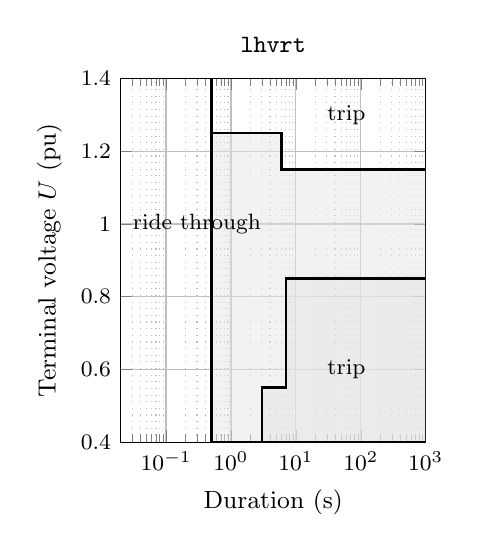
\begin{tikzpicture}
\begin{axis}[width=0.45\linewidth,height=62mm,xmode=log,xmin=0.02,xmax=1000,ymin=0.4,ymax=1.4,
  xlabel={Duration (s)},ylabel={Terminal voltage $U$ (pu)},grid=both,minor grid style={dotted},
  title={\texttt{lhvrt}},title style={font=\small},label style={font=\small},tick label style={font=\footnotesize}]
  \addplot[thick,const plot,fill=gray!20,fill opacity=0.5,draw=black] coordinates {(0.5,1.4) (0.5,1.25) (6,1.15) (1000,1.15) (1000,1.4)} \closedcycle;
  \addplot[thick,const plot,fill=gray!20,fill opacity=0.5,draw=black] coordinates {(3,0.4) (3,0.55) (7,0.85) (1000,0.85) (1000,0.4)} \closedcycle;
  \node[font=\footnotesize] at (axis cs:60,1.3) {trip};
  \node[font=\footnotesize] at (axis cs:60,0.6) {trip};
  \node[font=\footnotesize] at (axis cs:0.3,1.0) {ride through};
\end{axis}
\end{tikzpicture}\hfill
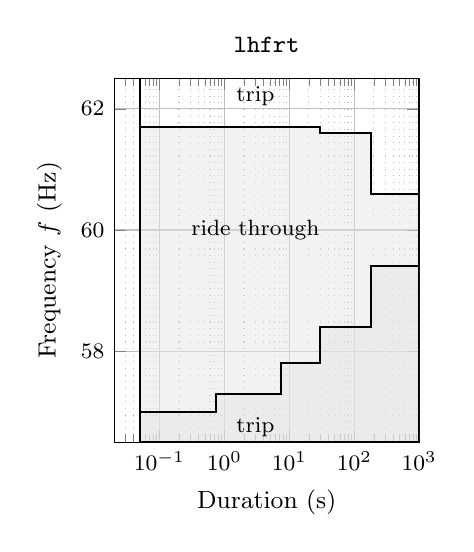
\begin{tikzpicture}
\begin{axis}[width=0.45\linewidth,height=62mm,xmode=log,xmin=0.02,xmax=1000,ymin=56.5,ymax=62.5,
  xlabel={Duration (s)},ylabel={Frequency $f$ (Hz)},grid=both,minor grid style={dotted},
  title={\texttt{lhfrt}},title style={font=\small},label style={font=\small},tick label style={font=\footnotesize}]
  \addplot[thick,const plot,fill=gray!20,fill opacity=0.5,draw=black] coordinates {(0.05,62.5) (0.05,61.7) (30,61.6) (180,60.6) (1000,60.6) (1000,62.5)} \closedcycle;
  \addplot[thick,const plot,fill=gray!20,fill opacity=0.5,draw=black] coordinates {(0.05,56.5) (0.05,57.0) (0.75,57.3) (7.5,57.8) (30,58.4) (180,59.4) (1000,59.4) (1000,56.5)} \closedcycle;
  \node[font=\footnotesize] at (axis cs:3,62.2) {trip};
  \node[font=\footnotesize] at (axis cs:3,56.75) {trip};
  \node[font=\footnotesize] at (axis cs:3,60) {ride through};
\end{axis}
\end{tikzpicture}
\caption{Must-trip regions (shaded) defined by the \texttt{lhvrt} and \texttt{lhfrt} settings. A unit trips once the terminal quantity has remained inside a shaded region for the duration on the abscissa.}
\label{fig:rt}
\end{figure}
